% Copyright 2021  Ed Bueler

\documentclass[10pt,hyperref,dvipsnames]{beamer}

\mode<presentation>{
  \usetheme{Madrid}
  \usecolortheme{beaver}
  \setbeamercovered{transparent}
  \setbeamerfont{frametitle}{size=\large}
}

\setbeamercolor*{block title}{bg=red!10}
\setbeamercolor*{block body}{bg=red!5}

\usepackage[english]{babel}
\usepackage[latin1]{inputenc}
\usepackage{times}
\usepackage[T1]{fontenc}
% Or whatever. Note that the encoding and the font should match. If T1
% does not look nice, try deleting the line with the fontenc.

\usepackage{amssymb,pifont}
\usepackage{empheq}
\usepackage{xspace}
\usepackage{verbatim,fancyvrb}

\usepackage{tikz}
\usetikzlibrary{shapes,arrows.meta,decorations.markings,decorations.pathreplacing,fadings,positioning}

\usepackage{hyperref}

% If you wish to uncover everything in a step-wise fashion, uncomment
% the following command:
%\beamerdefaultoverlayspecification{<+->}

\newcommand{\ba}{\mathbf{a}}
\newcommand{\bb}{\mathbf{b}}
\newcommand{\bc}{\mathbf{c}}
\newcommand{\bbf}{\mathbf{f}}
\newcommand{\bg}{\mathbf{g}}
\newcommand{\bn}{\mathbf{n}}
\newcommand{\bq}{\mathbf{q}}
\newcommand{\br}{\mathbf{r}}
\newcommand{\bx}{\mathbf{x}}
\newcommand{\by}{\mathbf{y}}
\newcommand{\bv}{\mathbf{v}}
\newcommand{\bu}{\mathbf{u}}
\newcommand{\bw}{\mathbf{w}}

\newcommand{\bF}{\mathbf{F}}
\newcommand{\bG}{\mathbf{G}}
\newcommand{\bQ}{\mathbf{Q}}

\newcommand{\bzero}{\mathbf{0}}

\newcommand{\grad}{\nabla}
\newcommand{\Div}{\nabla\cdot}
\newcommand{\minmod}{\operatorname{minmod}}

\newcommand{\CC}{\mathbb{C}}
\newcommand{\RR}{\mathbb{R}}

\newcommand{\ddt}[1]{\ensuremath{\frac{\partial #1}{\partial t}}}
\newcommand{\ddx}[1]{\ensuremath{\frac{\partial #1}{\partial x}}}
\newcommand{\Matlab}{\textsc{Matlab}\xspace}
\newcommand{\Octave}{\textsc{Octave}\xspace}
\newcommand{\eps}{\epsilon}

\newcommand{\ip}[2]{\left<#1,#2\right>}

\newcommand{\trefcolumn}[1]{\begin{bmatrix} \phantom{x} \\ #1 \\ \phantom{x} \end{bmatrix}}
\newcommand{\trefmatrixtwo}[2]{\left[\begin{array}{c|c|c} & & \\ #1 & \dots & #2 \\ & & \end{array}\right]}
\newcommand{\trefmatrixthree}[3]{\left[\begin{array}{c|c|c|c} & & & \\ #1 & #2 & \dots & #3 \\ & & & \end{array}\right]}
\newcommand{\trefmatrixgroups}[4]{\left[\begin{array}{c|c|c|c|c|c} & & & & & \\ #1 & \dots & #2 & #3 & \dots & #4 \\ & & & & & \end{array}\right]}

\newcommand{\blocktwo}[4]{\left[\begin{array}{c|c} #1 & #2 \\ \hline #3 & #4 \end{array}\right]}

\newcommand{\cmark}{\ding{51}}
\newcommand{\xmark}{\ding{55}}

\newcommand{\rhoi}{\rho_{\text{i}}}

\newcommand{\ds}{\displaystyle}


\title{Stokes problems using Firedrake}

\subtitle{A glacier and ice sheet tutorial}

\author{Ed Bueler}

\institute[UAF]{University of Alaska Fairbanks}

\date[April 2021]{April 2021  \\ \phantom{foo} \\ \phantom{foo} \\
\large \href{https://github.com/bueler/stokes-ice-tutorial}{\alert{\texttt{github.com/bueler/stokes-ice-tutorial}}} }


\begin{document}
\beamertemplatenavigationsymbolsempty

\begin{frame}
  \maketitle
\end{frame}

\begin{frame}
  \frametitle{Outline}

\centerline{\large \href{https://github.com/bueler/stokes-ice-tutorial}{\alert{\texttt{github.com/bueler/stokes-ice-tutorial}}}}

\bigskip
  \tableofcontents[hideallsubsections]
\end{frame}

\begin{frame}{exclamation points}

\begin{itemize}
\item \alert{I cannot explain everything in an hour!}

\item \alert{ask questions!}

\item \alert{please try the codes!}

\item \alert{feel free to send future questions by email!}
\end{itemize}
\end{frame}

\section{the problem and the equations}

\begin{frame}{the glacier \underline{dynamics} problem}

\begin{itemize}
\item conservation principles apply to ice sheets; each one is a PDE
    \begin{itemize}
    \item[$\circ$] mass \hfill \cmark\qquad today
    \item[$\circ$] momentum \hfill \cmark\qquad today
    \item[$\circ$] energy \hfill \xmark\,\, \emph{not today}
    \end{itemize}
\item Stokes model $=$ momentum conservation $+$ incompressibility
    \begin{itemize}
    \item[$\circ$] incompressibility is one aspect of mass conservation
    \item[$\circ$] no attempt \emph{today} to model geometry changes using surface balance, the other aspect
    \end{itemize}
\item \alert{the Stokes model determines velocity and pressure from given geometry}

\bigskip
{\scriptsize velocity} \hfill 
\includegraphics[width=0.85\textwidth]{figs/speed.png}

\bigskip
{\scriptsize pressure} \hfill 
\includegraphics[width=0.85\textwidth]{figs/pressure.png}

\bigskip
\end{itemize}
\end{frame}


\begin{frame}{Glen-Stokes equations}

\begin{columns}
\begin{column}{0.8\textwidth}
\begin{align*}
- \nabla \cdot \tau + \nabla p &= \rhoi \bg &&\text{\emph{stress balance}} \\
\nabla \cdot \bu &= 0 &&\text{\emph{incompressibility}} \\
\tau &= B_n |D\bu|^{(1/n) - 1} D\bu  &&\text{\emph{Glen flow law}}
\end{align*}
\end{column}

\begin{column}{0.2\textwidth}

\vspace{5mm}
%https://www.bl.uk/voices-of-science/interviewees/john-glen#
\hfill 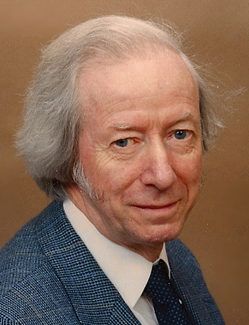
\includegraphics[width=0.6\textwidth]{figs/people/jglen.png}

\hfill {\tiny John Glen}
\end{column}
\end{columns}

\bigskip
\begin{itemize}
\item $\bu$ is velocity, $p$ is pressure, and $\tau$ is the deviatoric stress tensor
\item constants: {\small $\rhoi=910 \,\text{kg}\,\text{m}^{-3}$, $g=9.81\,\text{m}\,\text{s}^{-2}$, $n=3$, $B_n=6.8\times 10^7\,\text{Pa}\,\text{s}^{1/3}$}
\item viscosity regularization with $\eps = 10^{-4}$ and $D_0 = 1\,\text{a}^{-1}$:
\begin{equation*}
\nu_\eps(|D\bu|) = \frac{1}{2} B_n \left(|D\bu|^2 + \eps\, D_0^2\right)^{((1/n) - 1)/2}
\end{equation*}
\item eliminate $\tau$ to give system for $\bu,p$:
\begin{align*}
- \nabla \cdot \left(2 \nu_\eps(|D\bu|)\, D\bu\right) + \nabla p &= \rhoi \mathbf{g} && \text{\emph{momentum conservation}} \\
\Div \bu &= 0 && \text{\emph{(bulk) mass conservation}}
\end{align*}
\end{itemize}
\end{frame}


\begin{frame}{boundary conditions, as simple as possible}

\begin{itemize}
\item stress-free top:
\begin{equation*}
\sigma \bn = \left(2 \nu_\eps(|D\bu|) D\bu - pI\right) \bn = \bzero
\end{equation*}

\bigskip

\includegraphics[width=0.9\textwidth]{figs/speed.png}

\bigskip
\item no slip base:
\begin{equation*}
\bu = \bzero
\end{equation*}
    \begin{itemize}
    \item[$\circ$] no attempt \emph{today} to model sliding
    \end{itemize}
\end{itemize}
\end{frame}


\begin{frame}{the linear Stokes equations}

\begin{columns}

\begin{column}{0.6\textwidth}
\begin{itemize}
\item if we make viscosity constant ($\nu_0$) then we get the linear Stokes system:
\begin{align*}
- \nabla \cdot \left(2 \nu_0\, D\bu\right) + \nabla p &= \rhoi \mathbf{g}  \\
\Div \bu &= 0
\end{align*}
\item with reformatting:
\begin{align*}
- \nu_0 \nabla^2 \bu + \nabla p &= \rhoi \mathbf{g}  \\
-\Div \bu \qquad \,\,\,\, &= 0
\end{align*}
\item it has symmetric block structure
  $$\begin{bmatrix} A & B^\top \\ B & 0 \end{bmatrix} \begin{bmatrix} \bu \\ p  \end{bmatrix} = \begin{bmatrix} \bbf \\ 0 \end{bmatrix}$$
\end{itemize}
\end{column}

\begin{column}{0.4\textwidth}
\hfill 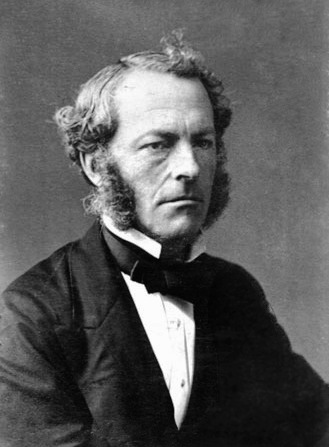
\includegraphics[width=0.4\textwidth]{figs/people/gstokes.jpg}

\hfill {\tiny George Stokes}

\vspace{7mm}
\hfill 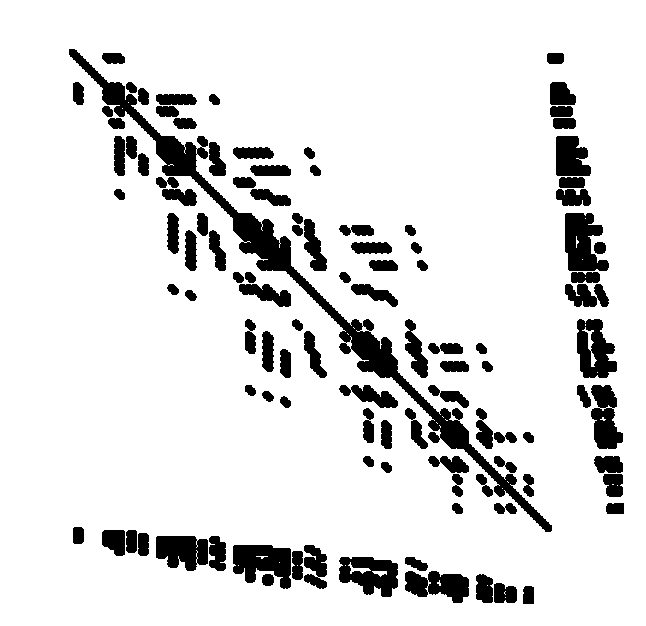
\includegraphics[width=0.8\textwidth]{figs/Kstokes.pdf}
\end{column}

\end{columns}
\end{frame}


\begin{frame}{finite elements \dots with no details}

\begin{itemize}
\item exact solution of the Stokes model is impossible for most geometries
    \begin{itemize}
    \item[$\circ$] slab-on-a-slope is an exception
    \end{itemize}
\item so we solve numerically using the finite element (FE) method
    \begin{itemize}
    \item[$\circ$] \alert{the whole point of Firedrake is that we \emph{don't} need to know the details of FE}
    \end{itemize}
\item in summary, the FE method allow us to start from a mesh of triangles {\small (or quadrilaterals, prisms, \dots) over our domain, {\footnotesize then express the approximate solution in terms of functions built from the mesh, {\scriptsize then turn the \alert{weak form} of the equations into a finite system by using test functions built from the mesh, {\tiny and then solve those equations somehow, and then there is a lot of fine print lorem ipsum dolor sit amet consectetur adipiscing elit etiam ex neque rhoncus a nunc tristique dignissim euismod magna fusce pharetra tempor sapien vitae scelerisque duis in quam rhoncus suscipit leo quis pellentesque diam suspendisse mollis nisi et eros ornare tincidunt maecenas sed pellentesque ex id mattis libero morbi erat orci fermentum eu dui ac \dots}}}}

\medskip
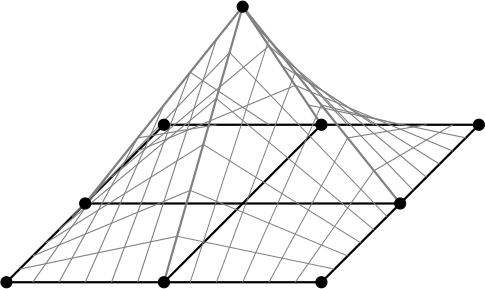
\includegraphics[width=0.2\textwidth]{figs/hat.png} \hfill

\vspace{-9mm}
\hfill 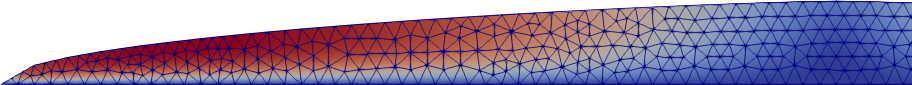
\includegraphics[width=0.7\textwidth]{figs/stage2.png}

\bigskip
\item we need to write a \alert{weak form}!
\end{itemize}
\end{frame}


\begin{frame}[fragile]
\frametitle{weak form}

\begin{itemize}
\item start from the original equations, also called the \emph{strong form}:
\small
\begin{align}
- \nabla \cdot \left(2 \nu_\eps(|D\bu|)\, D\bu\right) + \nabla p &= \rhoi \mathbf{g} \\
\Div \bu &= 0
\end{align}
\normalsize
\item multiply (1) by test velocity $\bv$ and (2) by test pressure $q$, integrate by parts, and combine into one nonlinear residual function:
    $$F(\bu,p;\bv,q) = \int_{\Omega} 2 \nu_\eps(|D\bu|)\, D\bu\,:\,D\bv - p \nabla \cdot \bv - q \nabla \cdot \bu - \rhoi \mathbf{g} \cdot \bv \,dx$$
\item in Firedrake's language (= \emph{Unified Form Language}) it looks like:

\medskip
\begin{Verbatim}[fontsize=\small]
fbody = Constant((0.0, 0.0, - rho * g))
Du2 = 0.5 * inner(D(u), D(u)) + (eps * Dtyp)**2.0
nu = 0.5 * Bn * Du2**((1.0 / n - 1.0)/2.0)
F = ( inner(2.0 * nu * D(u), D(v)) \
      - p * div(v) - q * div(u) - inner(fbody, v) ) * dx
\end{Verbatim}

\medskip
\item the actual weak form ``equation'' is the statement
   $$F(\bu,p;\bv,q) = 0 \qquad \text{ for all } \bv \text{ and } q$$
\end{itemize}
\end{frame}


\begin{frame}[fragile]
\frametitle{mixed finite elements for fluid problems}

\begin{itemize}
\item the other detail we need to know about in practice:

\bigskip
\begin{center}
\alert{choose separate function spaces for the velocity and the pressure}
\end{center}

\bigskip
\begin{center}
and
\end{center}

\bigskip
\begin{center}
\alert{choose spaces that the experts say are ``stable''}
\end{center}

\bigskip
\item Firedrake makes this elegant:

\medskip
\begin{Verbatim}[fontsize=\small]
V = VectorFunctionSpace(mesh, 'Lagrange', 2)   # u space
W = FunctionSpace(mesh, 'Lagrange', 1)         # p space
Z = V * W
up = Function(Z)
u, p = split(up)
v, q = TestFunctions(Z)
\end{Verbatim}
\end{itemize}
\end{frame}


\section{\texttt{stage1/} \qquad linear Stokes}

\begin{frame}[fragile]
\frametitle{running Firedrake programs}

\begin{itemize}
\item now I'm actually going to run some Python Firedrake code!
\item install Firedrake following these directions:

\begin{center}
\href{https://www.firedrakeproject.org/download.html}{\texttt{firedrakeproject.org/download.html}}
\end{center}
\item activate the Python virtual environment every time you use Firedrake:

\bigskip
\begin{Verbatim}
$ unset PETSC_DIR; unset PETSC_ARCH;  # may be needed
$ source ~/firedrake/bin/activate
\end{Verbatim}

\bigskip
    \begin{itemize}
    \item[$\circ$] I use an alias \texttt{drakeme} for this
    \end{itemize}

\bigskip
\item other tools I will need:
    \begin{itemize}
    \item[$\circ$] Gmsh \quad \href{https://gmsh.info/}{\texttt{gmsh.info}}
    \item[$\circ$] Paraview \quad \href{https://www.paraview.org/}{\texttt{paraview.org}}
    \end{itemize}

\bigskip
\item also grab my tutorial (codes and slides):
\small
\begin{center}
\texttt{git clone https://github.com/bueler/stokes-ice-tutorial.git}
\end{center}

\end{itemize}
\end{frame}


\begin{frame}[fragile]
\frametitle{\texttt{stage1/} \qquad linear Stokes}

\begin{itemize}
\item \emph{purpose:} solve linear Stokes on a trapezoidal glacier

    \begin{itemize}
    \item[$\circ$] simplified weak form
    \end{itemize}
{\small
    $$F(\bu,p;\bv,q) = \int_{\Omega} 2 \nu_0\, D\bu\,:\,D\bv - p \nabla \cdot \bv - q \nabla \cdot \bu - \rhoi \mathbf{g} \cdot \bv \,dx$$
}
\item \emph{source files:} \texttt{domain.geo}, \texttt{solve.py} \hfill \alert{$\gets$ inspect these!}
\item \emph{generated files:} \texttt{domain.msh}, \texttt{domain\_0.vtu}, \texttt{domain.pvd}
\end{itemize}

\bigskip
\begin{Verbatim}
$ cd stage1/
$ gmsh -2 domain.geo             # mesh the domain
$ gmsh domain.msh                # view the mesh
$ ./solve.py                     # solve linear Stokes
$ paraview domain.pvd            # view the solution
\end{Verbatim}
%$

\vspace{5mm}
\begin{center}

\includegraphics[width=0.9\textwidth]{figs/stage1.png}

{\tiny speed $|\bu|$}
\end{center}
\end{frame}


\section{\texttt{stage2/} \qquad Glen-Stokes}

\begin{frame}{Newton's method}

\begin{columns}
\begin{column}{0.8\textwidth}
\begin{itemize}
\item linear Stokes \small (\texttt{stage1/}) \normalsize needs only a single linear system:
  $$\begin{bmatrix} A & B^\top \\ B & 0 \end{bmatrix} \begin{bmatrix} \bu \\ p  \end{bmatrix} = \begin{bmatrix} \bbf \\ 0 \end{bmatrix}$$
    \begin{itemize}
    \item[$\circ$] Firedrake asks PETSc's KSP component to solve this
    \end{itemize}
\item but for Glen-Stokes the weak form is nonlinear in $\bu$:
\small
$$F(\bu,p;\bv,q) = \int_{\Omega} 2\, \alert{\nu_\eps(|D\bu|)\, D\bu}\,:\,D\bv - p \nabla \cdot \bv - q \nabla \cdot \bu - \rhoi \mathbf{g} \cdot \bv \,dx$$
\normalsize
\item Firedrake automatically applies Newton's method
    \begin{itemize}
    \item[$\circ$] because we write \texttt{solve(F == 0,}\dots
    \end{itemize}
\item all you need to know about Newton's iteration:
    \begin{itemize}
    \item[$\circ$] it is repeated linearization around the current iterate
    \item[$\circ$] Firedrake uses UFL symbolic differentiation for linearization
    \item[$\circ$] Firedrake asks PETSc's SNES to do the Newton iteration
        \begin{itemize}
        \item SNES options will monitor and control the Newton iteration
        \end{itemize}
    \end{itemize}
\end{itemize}
\end{column}
\begin{column}{0.2\textwidth}
\vspace{25mm}

\hfill 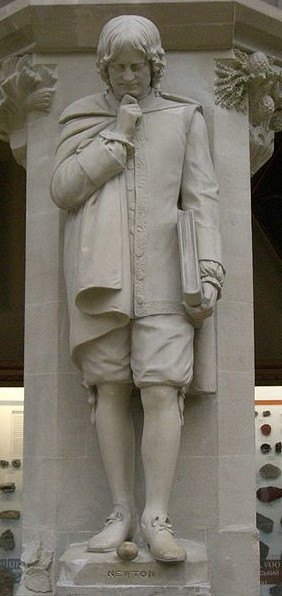
\includegraphics[width=0.8\textwidth]{figs/people/inewton.jpg}

\hfill {\tiny Isaac Newton}
\end{column}
\end{columns}
\end{frame}


\begin{frame}[fragile]
\frametitle{\texttt{stage2/} \qquad Glen-Stokes}

\begin{itemize}
\item \emph{purpose:} solve Glen-Stokes on a flat-bed glacier
\item \emph{source files:} \texttt{domain.py}, \texttt{solve.py} \hfill \alert{$\gets$ inspect these!}
\item \emph{generated files:} \texttt{dome.geo}, \texttt{dome.msh}, \texttt{dome\_0.vtu}, \texttt{dome.pvd}
\end{itemize}

\bigskip
\begin{Verbatim}
$ cd stage2/
$ ./domain.py                   # generate geometry
$ gmsh -2 dome.geo              # mesh domain
$ gmsh dome.msh                 # view mesh
$ ./solve.py -s_snes_monitor -s_snes_converged_reason
$ paraview dome.pvd             # view solution
\end{Verbatim}

\vspace{10mm}
\begin{center}
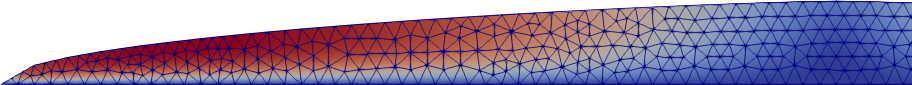
\includegraphics[width=0.9\textwidth]{figs/stage2.png}

{\tiny speed $|\bu|$}
\end{center}
\end{frame}


\section{\texttt{stage3/} \qquad extruded meshes}

\begin{frame}[fragile]
\frametitle{\texttt{stage3/} \qquad extruded meshes}

\begin{itemize}
\item \emph{purpose:} solve same problem using an extruded quadrilateral mesh
\item \emph{source files:} \texttt{solve.py} \hfill \alert{$\gets$ inspect this!}
\item \emph{generated files:} \texttt{dome\_0.vtu}, \texttt{dome.pvd}
\end{itemize}

\bigskip
\begin{Verbatim}
$ cd stage3/
$ ./solve.py -s_snes_monitor -s_snes_converged_reason
$ paraview dome.pvd
\end{Verbatim}
%$

\vspace{10mm}
\begin{center}
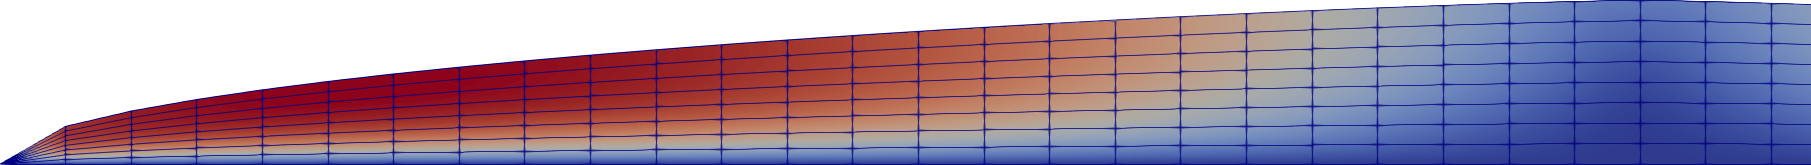
\includegraphics[width=0.9\textwidth]{figs/stage3.png}

{\tiny speed $|\bu|$}
\end{center}
\end{frame}


\begin{frame}[fragile]
\frametitle{convergence?}

\begin{itemize}
\item \texttt{stage3/} code \texttt{solve.py} allows adjustable resolution, e.g.:
\begin{Verbatim}
$ ./solve.py -mx 40 -mz 4
\end{Verbatim}
%$
\item velocity results are reasonable and consistent:

\medskip
% timer ./solve.py -s_snes_rtol 1.0e-5 -s_snes_max_it 200 -s_snes_converged_reason -mx MX -mz MZ
% timer ./solve.py -s_snes_rtol 1.0e-5 -s_snes_max_it 200 -s_snes_converged_reason -mx 640 -mz 64 -eps 0.01
\begin{center}
\small
\begin{tabular}{c|rrr}
mesh           &   $\Delta x\times \Delta z$ (m) & av.~$|\bu|$ (m/a) & max.~$|\bu|$ (m/a) \\ \hline
$20\times 2$   &  $1000 \times 500$ &        1813 &         3512 \\
$40\times 4$   &   $500 \times 250$ &        1787 &         3293 \\
$80\times 8$   &   $250 \times 125$ &        1769 &         3223 \\
$160\times 16$ &    $125 \times 63$ &        1762 &         3199 \\
$320\times 32$ &     $63 \times 31$ &        1759 &         3191 \\
$640\times 64$ &     $31 \times 16$ &        1758 &         3190
\end{tabular}
\normalsize
\end{center}

    \begin{itemize}
    \item[$\circ$] \emph{unfortunately}, the finest resolution needed $\eps=10^{-2}$ to get ``unstuck'' from the $\bu,p=\mathbf{0},0$ initial iterate
    \end{itemize}
\item we need \alert{better initial iterates} for high-resolution runs
\end{itemize}
\end{frame}


\section{\texttt{stage4/} \qquad bells and whistles}

\begin{frame}[fragile]
\frametitle{\texttt{stage4/} \qquad bells and whistles}

\begin{itemize}
\item \emph{purpose:} additional robust and/or useful features
    \begin{itemize}
    \item[$\circ$] rescale the equations  \hfill \emph{better conditioning}
    \item[$\circ$] vertical grid sequencing  \hfill \emph{better initial iterates}
    \item[$\circ$] $100\eps$ on coarse meshes in sequencing  \hfill \emph{better initial iterates}
    \item[$\circ$] generate stress tensor $\tau$ from solution  \hfill \emph{diagnostic}
    \item[$\circ$] generate effective viscosity $\nu_\eps$ from solution  \hfill \emph{diagnostic}
    \end{itemize}
\item \emph{source files:} \texttt{solve.py} \hfill \alert{$\gets$ inspect this!}
\item \emph{generated files:} \texttt{dome\_0.vtu}, \texttt{dome.pvd}
\end{itemize}

\bigskip
\begin{Verbatim}
$ cd stage4/
$ ./solve.py
$ ./solve.py -mx 320 -mz 2 -refine 2 \
    -s_snes_atol 1.0e-2 -s_snes_monitor
$ paraview dome.pvd
\end{Verbatim}
%$

\bigskip
\begin{center}

\includegraphics[width=0.9\textwidth]{figs/stage4.png}

{\tiny deviatoric stress magnitude $\|\tau\|$}
\end{center}
\end{frame}


\section{\texttt{stage5/} \qquad 3D glaciers in parallel}

\begin{frame}[fragile]
\frametitle{\texttt{stage5/} \qquad 3D glaciers in parallel}

\begin{itemize}
\item \emph{purpose:} 3D ice sheet in parallel on bumpy bed
\item \emph{source files:} \texttt{solve.py} \hfill \alert{$\gets$ inspect this!}
\item \emph{generated files:} \texttt{dome\_0\_}$k$\texttt{.vtu}, \texttt{dome\_0.pvtu}, \texttt{dome.pvd}
\end{itemize}

\bigskip
\begin{Verbatim}
$ cd stage5/
$ mpiexec -n 4 ./solve.py -refine 0 \
    -s_snes_atol 1.0e-2 -s_snes_monitor
$ paraview dome.pvd
$ mpiexec -n 12 ./solve.py -bumpy -baserefine 5 \
    -refine 2 -s_snes_atol 1.0e-2 -s_snes_monitor \
    -o hires.pvd
$ paraview hires.pvd
\end{Verbatim}
%$

\bigskip
\begin{center}
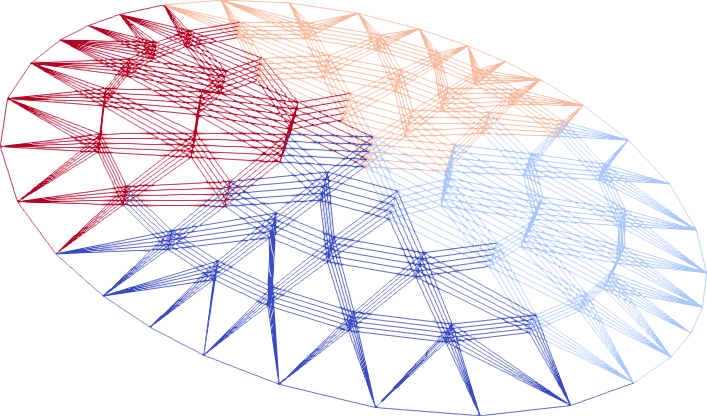
\includegraphics[width=0.4\textwidth]{figs/stage5.png}
\end{center}
\end{frame}


\begin{frame}{learn more}

\centerline{\large \href{https://github.com/bueler/stokes-ice-tutorial}{\alert{\texttt{github.com/bueler/stokes-ice-tutorial}}}}

\medskip
\hrulefill


\begin{columns}
\begin{column}{0.6\textwidth}
\small

\begin{itemize}
\item Firedrake: \href{https://www.firedrakeproject.org/}{\texttt{firedrakeproject.org}}

    \begin{itemize}
    \scriptsize
    \item tutorials \& manual: \href{https://www.firedrakeproject.org/documentation.html}{\texttt{.../documentation.html}}
    \item Jupyter notebooks page: \href{https://www.firedrakeproject.org/notebooks.html}{\texttt{.../notebooks.html}}
    \end{itemize}
\item PETSc website: \href{https://www.mcs.anl.gov/petsc/}{\texttt{www.mcs.anl.gov/petsc}}
\item for Glen-Stokes eqns, see Ch.~1 by Hewitt:


{\scriptsize Fowler \& Ng, ed., \emph{Glaciers and Ice Sheets in the Climate System: The Karthaus Summer School Lecture Notes}, Springer 2021}

\item for finite elements and linear Stokes:

{\scriptsize Elman, Silvester, \& Wathen, \emph{Finite Elements and Fast Iterative Solvers, With Applications in Incompressible Fluid Dynamics}, Oxford 2014, 2nd ed.}

\item for PETSc, Firedrake, and Stokes (Ch.~14):

{\scriptsize Bueler, \emph{PETSc for Partial Differential Equations: Numerical Solutions in C and Python}, SIAM 2021}
\end{itemize}
\end{column}

\begin{column}{0.4\textwidth}

\bigskip
\href{https://www.firedrakeproject.org/}{
\includegraphics[width=\textwidth]{figs/firedrakebanner.png}}

\bigskip
\hfill \href{https://www.mcs.anl.gov/petsc/}{
\includegraphics[width=0.6\textwidth]{figs/petscbanner.png}}

\vspace{25mm}

\includegraphics[width=0.31\textwidth]{figs/covers/karthaus.png} \hfill
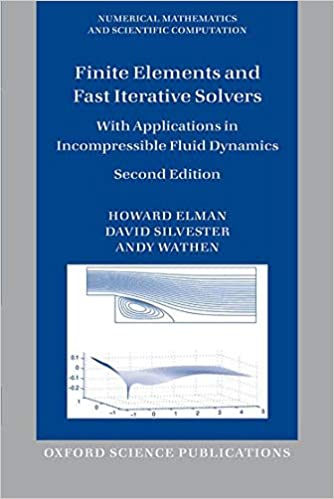
\includegraphics[width=0.31\textwidth]{figs/covers/elman.jpg} \hfill
\href{https://my.siam.org/Store/Product/viewproduct/?ProductId=32850137}{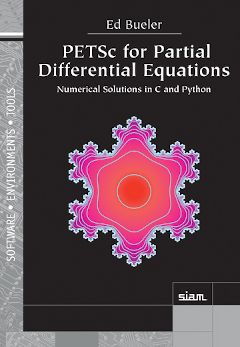
\includegraphics[width=0.32\textwidth]{figs/covers/bueler.jpg}}
\end{column}

\end{columns}
\end{frame}


\end{document}
